

\subsubsection{K-nearest neighbors}
To try and find the optimal K-nearest neighbors model, we looked $40 \times 4 = 160$ different models: All values of K (the number of nearest neighbors) between 1 and 40 and 4 different distance measures: Euclidean, cityblock, correlation, and cosine, where
% \vspace{-0.1cm}
% \begin{align}
% correlation(\vek{x},\vek{y}) &= 1 - \hat{\text{cor}}(\vek{x},\vek{y}) \\
% cosine(\vek{x},\vek{y}) &= 1 - \frac{\vek{x}^T\vek{y}}{\norm{\vek{x}}\norm{\vek{y}}},
% \end{align}
% \vspace{-0.1cm}

\vspace{-0.1cm}
\begin{equation}
correlation(\vek{x},\vek{y}) = 1 - \hat{\text{cor}}(\vek{x},\vek{y}),\;\;
cosine(\vek{x},\vek{y}) = 1 - \frac{\vek{x}^T\vek{y}}{\norm{\vek{x}}\norm{\vek{y}}},
\end{equation}
\vspace{-0.1cm}

with $\hat{\text{cor}}(\vek{x},\vek{y})$ being the correlation coefficient as defined in \cite[eq. 4.7]{ coursenotes}. It is chosen that the models will choose the nearest neighbor class in case of ties.

\begin{figure}[H]
    \centering
    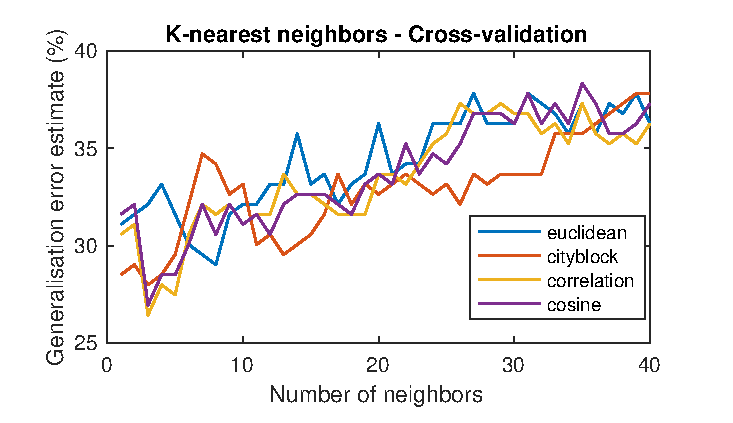
\includegraphics[width=0.52\textwidth]{fig/knn-crossval.eps}
    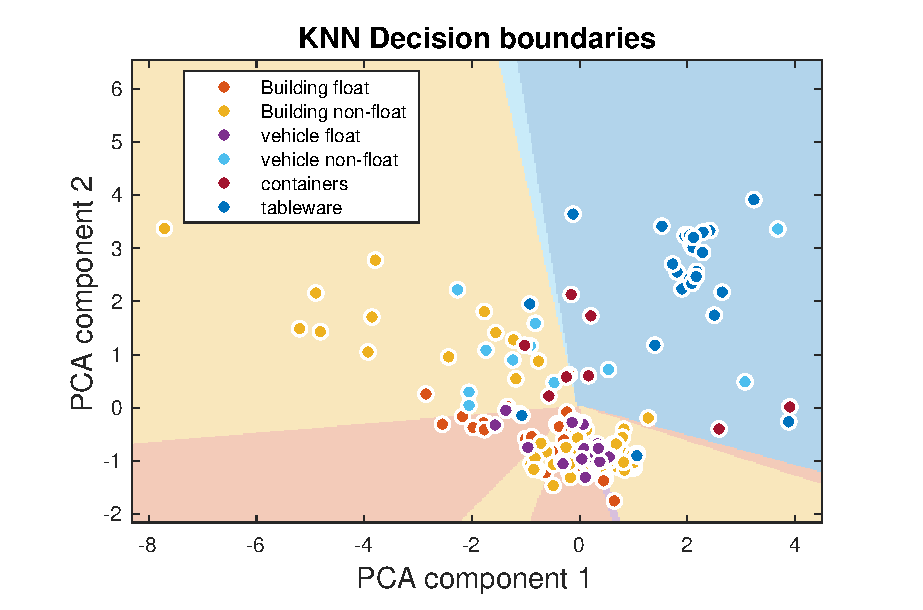
\includegraphics[width = 0.44\textwidth]{fig/knn-decision-bounds.eps}
    \caption{\textbf{Left:} Estimates of the generalization error for the K nearest neighbors model as a function of the number of neighbors for 3 different distance measures. The models are fitted to the training sets of the inner CV loop, and the generalization error estimate is the average of the error rate when these models are applied to the validation sets in the inner CV loops. \textbf{Right:} Decision bounds of the best K-nearest neighbor model fitted to the training set of the outer CV loop. The data points are also from the training set.}
    \label{knn-plots}
\end{figure}

From each of these models, we calculate and plot the estimates of their generalization error (figure \ref{knn-plots}) From each of the inner CV validation splits. The model with the smallest generalization error is then chosen as optimal, which is K=3 and the correlation distance. The model is then trained on the whole training set in the outer CV loop, and its decision boundaries projected onto the first principal components are plotted in Figure \ref{knn-plots}. Finally, an unbiased estimate of its generalization error is found by computing the classification error rate on the test set in the outer CV loop, which is shown in table \ref{classification-performance}.

It should be noted that, inspecting fig. \ref{knn-plots}., it is seen that the K=3 and the correlation distance is not convincingly the best model. The generalization error graphs are very spikey and noisy, suggesting that high variance is present in our cross-validation model. However, this is difficult to amend with the small amount of data (214 observations) that we are given. 